\section{A matched intervention in legal and scientific evidence}
\label{sec:natural-domains}
To test whether the historical suite atlas yields a source-independent stability conclusion, we separately froze a new, model-blind diagnostic from \emph{independent} natural-domain references: 144 document--hypothesis decisions from 91 ContractNLI test contracts \citep{contractnli}, and 120 claim--cited-abstract decisions from SciFact's labeled development set \citep{scifact}. The legal sample is balanced across entailment, contradiction and not-mentioned; the scientific sample is balanced across annotated support and contradiction. Each source pair receives an unchanged request, a byte-identical repeat, and a reversal of the candidate dictionary's insertion order. State, candidate meanings and reference label are invariant; no gold or source ID is sent to the models. All 792 requests were independently audited as complete for the four local adapters before inference; Jev's HTTP payload is complete, but server-side tokenization is not observable. We resample by contract or claim for pointwise 95\% intervals, and never combine the two domains into a prevalence-weighted score.

The paired state decomposition in Figure~\ref{fig:natural-domains} exposes information an accuracy table would discard. On legal inference, the two code-likelihood LLM adapters change 66/144 (Llama) and 64/144 (Qwen) selected labels under ordinary reversal. Llama's reference accuracy rises from 44/144 to 59/144, and Qwen's from 65/144 to 83/144, yet only 33/144 and 51/144, respectively, are reference-correct under \emph{both} renderings. These apparent gains are the net of 26 corrections versus 11 regressions for Llama and 32 versus 14 for Qwen. Their paired gains are $+10.4$ points (cluster interval $[+2.8,+18.3]$) and $+12.5$ points ($[+4.2,+20.7]$), respectively; they should not be read as better legal reasoning after a semantic change. In these adapters reversal also reassigns answer codes, so it is a joint model--interface perturbation; Section~\ref{sec:codebook} isolates its factors.

The same intervention has a different geometry on scientific evidence. Qwen changes 14/120 labels and loses eight net correct answers ($92/120\to84/120$; paired $-6.7$ points, $[-12.5,-0.8]$), while Jev remains reference-correct on the same 112/120 pairs under both orders. Jev's legal original/reversal agreement is 138/144, versus 142/144 on a literal repeat; all four local deterministic adapters have zero literal-repeat flips on these requests. Thus even the direction of the \emph{net} accuracy effect varies by domain and adapter, while joint correctness captures a more stable operational requirement. These are selected-pair descriptions, not a claim that the five systems' legal or scientific abilities are ranked across their native interfaces.

\begin{figure}[!t]
\centering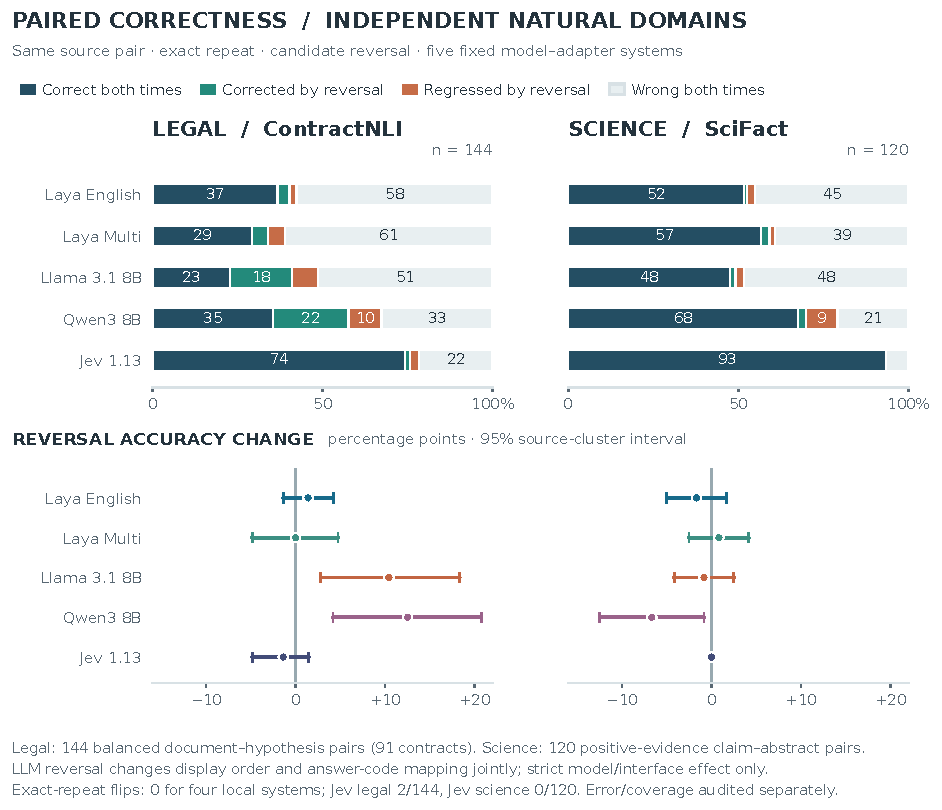
\includegraphics[width=.99\linewidth]{figures/fig_domain_expansion.pdf}
\caption{Paired correctness under candidate reversal on two independently sourced, deliberately class-balanced diagnostics. Each horizontal bar partitions the same source pairs into correct under both renderings, corrected, regressed and wrong under both; bars sum to 100\%. Lower panels show reversal minus base reference accuracy with pointwise 95\% contract- or claim-cluster intervals (10,000 draws). The LLM intervention changes display and code assignment jointly; codebook controls are separate. SciFact includes only positively annotated cited abstracts, not retrieval or no-information examples.}
\label{fig:natural-domains}
\end{figure}

Scope matters. The legal 16,000-character feasibility cap excludes 24/123 official test contracts and is format-selective; 48/144 contradiction cases in the selected diagnostic do not reflect the official test label prevalence. ContractNLI repeats 17 fixed hypotheses across documents. A document-blind lookup trained solely on the official training contracts' modal label for each hypothesis already attains 82/144 (56.9\%) on our frozen legal sample; it is a supervised shortcut diagnostic, not a fair zero-shot model baseline. SciFact's positive-evidence subset excludes no-information decisions and does not test retrieval; some contradiction claims originate from deliberate inversion of source claims. Source annotations are treated as references, not independently re-adjudicated truth. We report format/length and label-prior audits in Appendix~\ref{app:domain-validity}, and retain source attribution and reconstruction instructions in the companion artifact.
